\documentclass[multi={tikzpicture},border=8pt]{standalone}
\usepackage{tnviz}

\begin{document}

% 1. Line bonds run under the glyphs; ports leave a glyph along a direction.
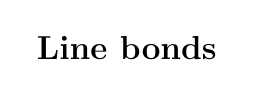
\begin{tikzpicture}[font=\sffamily]
  \node[font=\bfseries\large] at (2.6,2.2) {Line bonds};
  \tnvShape[shape=rounded rectangle,color=blue!64!black,width=16mm,height=11mm,corner radius=1.4mm,text color=white!92!black]{A}{(0,0)}{$A$}
  \tnvShape[shape=orb,color=orange!78!black,width=12mm]{B}{(2.6,0)}{$B$}
  \tnvShape[shape=diamond,color=violet!64!black,width=15mm,height=12mm,corner radius=1mm,text color=white!92!black]{C}{(5.2,0)}{$C$}
  \tnvBond{A}{B}
  \tnvBond{B}{C}
  \tnvBond[from=up,to=up,via={(0,1.4),(5.2,1.4)}]{A}{C}
  \tnvLeg{A}{down}{6mm}
  \tnvLeg{B}{down}{6mm}
  \tnvLeg{C}{down}{6mm}
\end{tikzpicture}

% 2. Straight tubes: the lit side follows the tube direction; open ends get
% hemispherical caps.
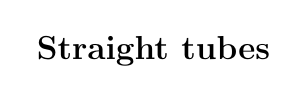
\begin{tikzpicture}[font=\sffamily]
  \node[font=\bfseries\large] at (2.6,2.4) {Straight tubes};
  \tnvShape[shape=rounded rectangle,color=blue!64!black,width=16mm,height=11mm,corner radius=1.4mm,text color=white!92!black]{A}{(0,0)}{$A$}
  \tnvShape[shape=orb,color=orange!78!black,width=12mm]{B}{(2.6,0)}{$B$}
  \tnvShape[shape=diamond,color=violet!64!black,width=15mm,height=12mm,corner radius=1mm,text color=white!92!black]{C}{(5.2,1.2)}{$C$}
  \tnvBond[style=tube]{A}{B}
  \tnvBond[style=tube,color=teal!60!black]{B}{C}
  \tnvLeg[style=tube]{A}{down}{7mm}
  \tnvLeg[style=tube]{B}{down}{7mm}
  \tnvLeg[style=tube,color=teal!60!black]{C}{-45}{7mm}
  \tnvLeg[style=tube,width=3.2mm,color=red!55!black]{A}{left}{6mm}
\end{tikzpicture}

% 3. Polyline tubes: every corner becomes a fillet and the lighting turns
% with the tube.
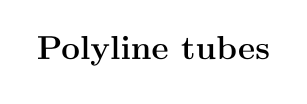
\begin{tikzpicture}[font=\sffamily]
  \node[font=\bfseries\large] at (2.6,2.6) {Polyline tubes};
  \tnvShape[shape=rounded rectangle,color=blue!64!black,width=16mm,height=11mm,corner radius=1.4mm,text color=white!92!black]{A}{(0,0)}{$A$}
  \tnvShape[shape=triangle,color=cyan!48!blue,width=15mm,height=12mm,corner radius=1mm,text color=white!92!black]{B}{(5.2,0)}{$B$}
  \tnvShape[shape=orb,color=orange!78!black,width=12mm]{C}{(2.6,-2.2)}{$C$}
  \tnvBond[style=tube,from=up,to=up,via={(0,1.6),(5.2,1.6)}]{A}{B}
  \tnvBond[style=tube,color=teal!60!black,from=down,via={(0,-2.2)}]{A}{C}
  \tnvBond[style=tube,color=red!55!black,from=down,to=right,via={(5.2,-1.35),(4.2,-1.35),(4.2,-2.2)}]{B}{C}
  \tnvBond[style=tube,width=3mm,color=black!45,from=left,bend radius=4mm,via={(-2.3,1.0),(-2.9,-0.4),(-1.9,-1.8)}]{A}{(-0.6,-2.6)}
\end{tikzpicture}

% 4. Crossings.  By default a crossing is left alone: the bond with the
% higher scene key (layer, z, source order) is simply drawn on top.
% crossing=hop makes that bond jump the crossing, as in circuit diagrams.
% Bonds may name glyphs that are placed later.
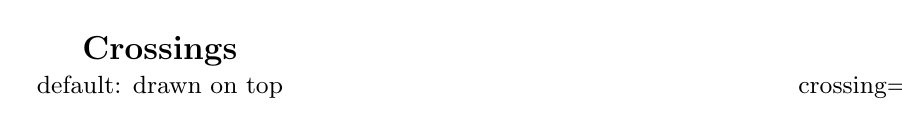
\begin{tikzpicture}[font=\sffamily]
  \node[font=\bfseries\large] at (3,3.0) {Crossings};
  \node[font=\small] at (3,2.55) {default: drawn on top};
  \tnvBond[style=tube,from=right,to=left]{P}{Q}
  \tnvBond[style=tube,color=teal!60!black,from=down,to=up]{R}{S}
  \tnvShape[shape=rounded rectangle,color=blue!64!black,width=12mm,height=9mm,corner radius=1.2mm,text color=white!92!black]{P}{(0,0.4)}{$P$}
  \tnvShape[shape=orb,color=orange!78!black,width=10mm]{Q}{(6,0.4)}{$Q$}
  \tnvShape[shape=diamond,color=violet!64!black,width=12mm,height=10mm,corner radius=1mm,text color=white!92!black]{R}{(3,2.0)}{$R$}
  \tnvShape[shape=triangle,color=cyan!48!blue,width=12mm,height=10mm,corner radius=1mm,text color=white!92!black]{S}{(3,-1.4)}{$S$}
  \tnvBond[via={(1.2,-0.8)}]{(0.2,-1.6)}{(1.8,1.4)}
  \tnvBond{(0.4,1.4)}{(1.6,-1.6)}

  \begin{scope}[xshift=8cm]
  \node[font=\small] at (3,2.55) {crossing=hop};
  \tnvBond[style=tube,from=right,to=left]{P2}{Q2}
  \tnvBond[style=tube,color=teal!60!black,from=down,to=up,crossing=hop]{R2}{S2}
  \tnvShape[shape=rounded rectangle,color=blue!64!black,width=12mm,height=9mm,corner radius=1.2mm,text color=white!92!black]{P2}{(0,0.4)}{$P$}
  \tnvShape[shape=orb,color=orange!78!black,width=10mm]{Q2}{(6,0.4)}{$Q$}
  \tnvShape[shape=diamond,color=violet!64!black,width=12mm,height=10mm,corner radius=1mm,text color=white!92!black]{R2}{(3,2.0)}{$R$}
  \tnvShape[shape=triangle,color=cyan!48!blue,width=12mm,height=10mm,corner radius=1mm,text color=white!92!black]{S2}{(3,-1.4)}{$S$}
  \tnvBond{(0.2,-1.0)}{(1.8,-1.0)}
  \tnvBond[crossing=hop]{(1.0,-1.6)}{(1.0,1.4)}
  \tnvBond[crossing=hop]{(4.4,-1.6)}{(5.6,1.4)}
  \tnvBond[style=tube,width=1.6mm,color=red!55!black,z=1,crossing=hop]{(3.8,-0.6)}{(5.8,-0.6)}
  \end{scope}
\end{tikzpicture}

% 5. Labels.  On a tube a label is printed along the axis and kept upright;
% beside a bond it stays upright and touches the bond from one side.  The
% position is a fraction of the visible length between the silhouettes.
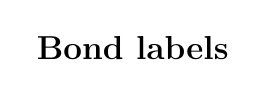
\begin{tikzpicture}[font=\sffamily]
  \node[font=\bfseries\large] at (3.4,2.9) {Bond labels};
  \tnvShape[shape=rounded rectangle,color=blue!64!black,width=13mm,height=10mm,corner radius=1.2mm,text color=white!92!black]{A}{(0,0)}{$A$}
  \tnvShape[shape=orb,color=orange!78!black,width=11mm]{B}{(3.4,0)}{$B$}
  \tnvShape[shape=diamond,color=violet!64!black,width=13mm,height=11mm,corner radius=1mm,text color=white!92!black]{C}{(6.8,0)}{$C$}
  \tnvShape[shape=triangle,color=cyan!48!blue,width=13mm,height=11mm,corner radius=1mm,text color=white!92!black]{D}{(3.4,-2.6)}{$D$}
  % On the tube (the default for tubes).
  \tnvBond[style=tube,width=3.2mm,label=$\chi$]{A}{B}
  \tnvBond[style=tube,width=3.2mm,color=teal!60!black,label=$\chi^2$]{C}{B}
  % Beside the tube, on either side.
  \tnvBond[style=tube,from=up,to=up,via={(0,1.9),(6.8,1.9)},label=$d$,label placement=beside]{A}{C}
  \tnvBond[style=tube,color=red!55!black,from=down,to=left,via={(0,-2.6)},label=$D_1$,label placement=beside,label side=right,label pos=.3]{A}{D}
  % Lines: beside by default.
  \tnvBond[to=right,from=down,via={(6.8,-2.6)},label=$k$]{C}{D}
  \tnvBond{B}{D}
  \tnvBond[label=$m$,label side=left]{(1.6,-3.8)}{(5.2,-3.8)}
  \tnvLeg[style=tube,width=3mm,color=black!45,label=$\sigma$]{C}{-30}{9mm}
\end{tikzpicture}

\end{document}
